\documentclass[border=2pt]{standalone}
\usepackage{pgfplots}
\usepgfplotslibrary{statistics}
\pgfplotsset{compat=1.18}
\begin{document}
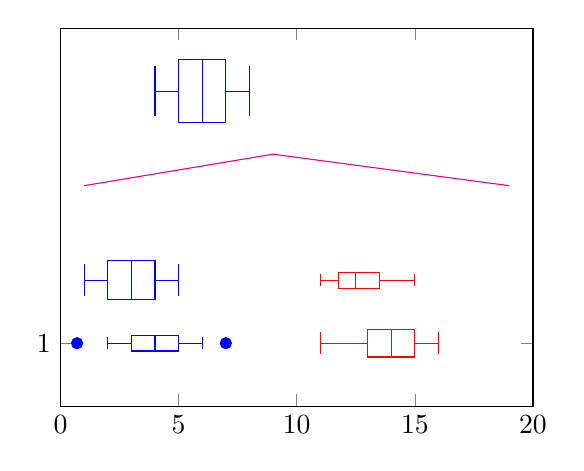
\begin{tikzpicture}
\begin{axis}[
    width=60mm,height=48mm,scale only axis,
    xmin=0,xmax=20,ymin=0,ymax=6,xtick={0,5,10,15,20},ytick=data,
    boxplot/variable width,boxplot/box extend=1,boxplot/variable width min target=0.25,
    boxplot/sample size min=4,boxplot/sample size max=36,
]
    \addplot[blue,mark=*,boxplot prepared={sample size=4,
        lower whisker=2,lower quartile=3,median=4,upper quartile=5,upper whisker=6}]
        coordinates {(0,0.7) (0,7)};
    \addplot[magenta,no marks] coordinates {(1,3.5) (9,4) (19,3.5)};
    \addplot[red,boxplot] coordinates {
        (0,14) (0,12) (0,15) (0,13) (0,11) (0,16) (0,14) (0,15) (0,13)};
    \addplot[blue,boxplot prepared={sample size=16,
        lower whisker=1,lower quartile=2,median=3,upper quartile=4,upper whisker=5}]
        coordinates {};
    \addplot[red,boxplot] coordinates {(0,12) (0,15) (0,11) (0,13)};
    \addplot[blue,boxplot prepared={draw position=5,sample size=36,
        lower whisker=4,lower quartile=5,median=6,upper quartile=7,upper whisker=8}]
        coordinates {};
\end{axis}
\end{tikzpicture}
\end{document}
